\section{Model Experiments and Results}
\label{sec: modelresults}

\subsection{Capture learning trajectories via model fitting and ablation}

Our modular Bayesian framework can simulate a wide range of learning dynamics, allowing us to isolate latent factors that shape individuals’ learning behavior. Fig.~\ref{fig:3}A–B summarizes model performance across eight candidate variants using the two metrics introduced in Section \ref{sec:3.3}. While the full model (HPM) shows comparable external performance to several reduced models (M, PM, MH, and PMH), it outperforms them markedly in capturing internal representations (** indicates FDR-corrected $p < 0.01$). 

% \vspace{1em}
\begin{figure}[htp!]
  \centering
  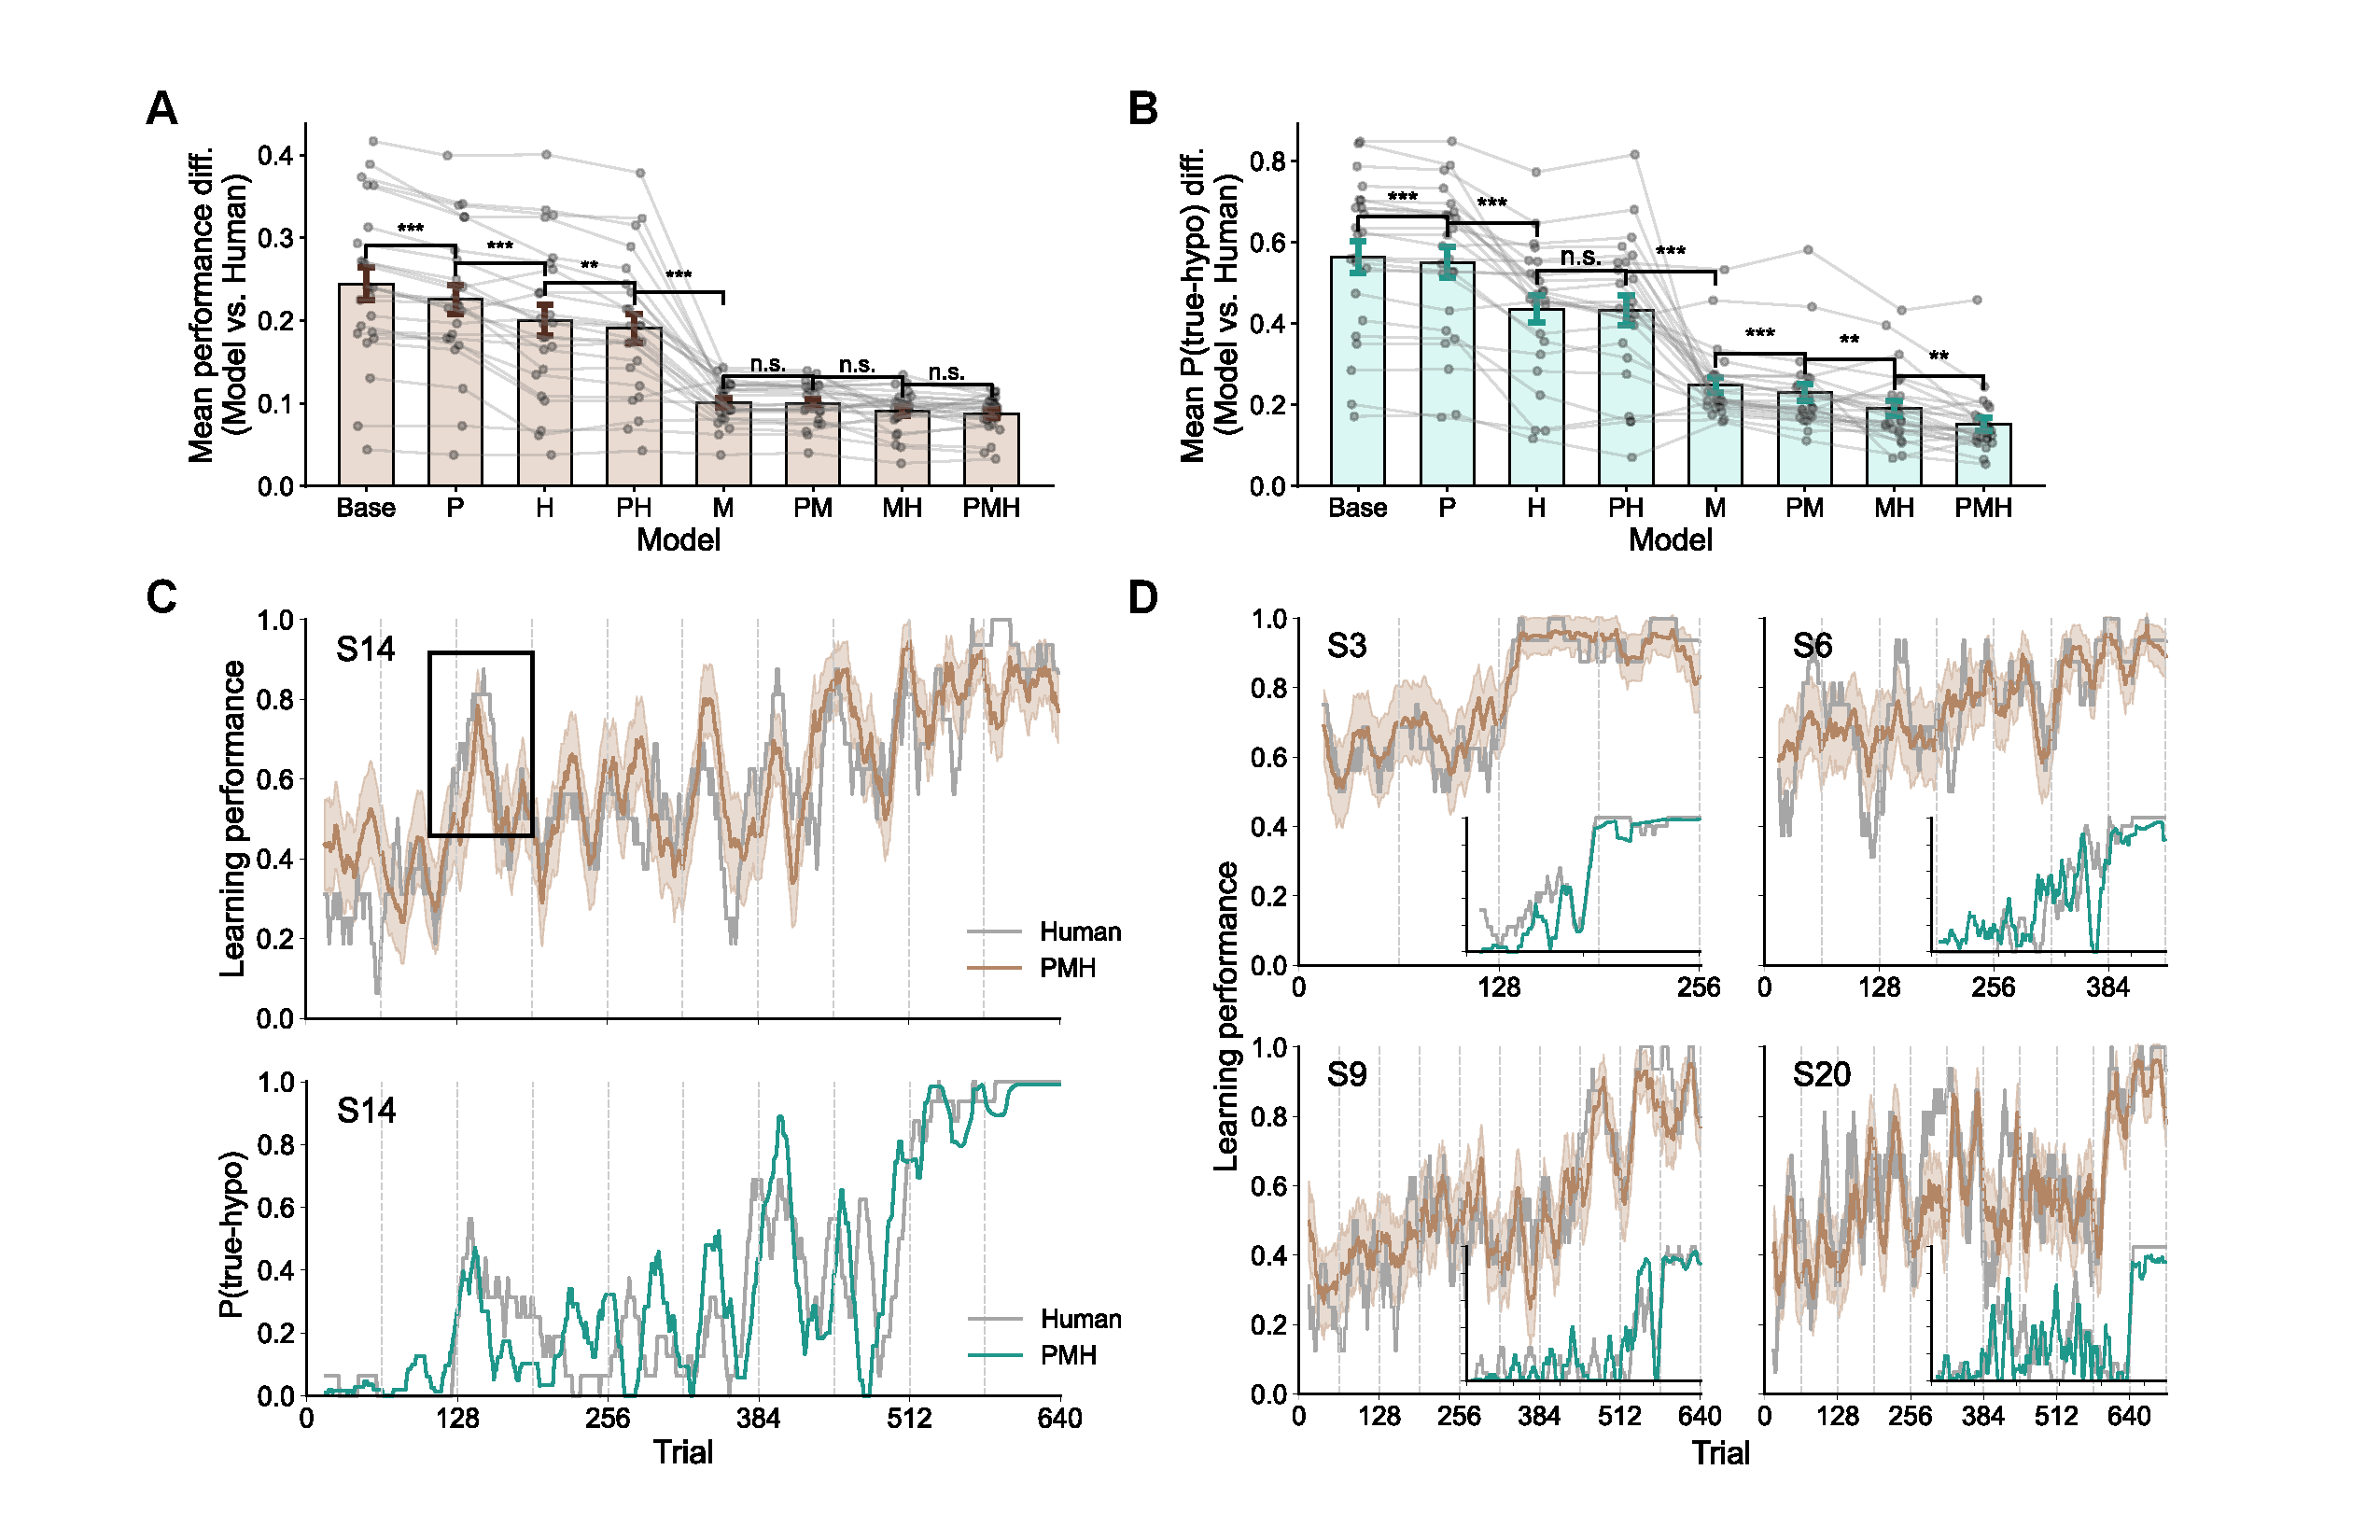
\includegraphics[width=1\textwidth, trim=2.6cm 1.3cm 3.5cm 1.5cm, clip]{figs/Figure3.pdf}
  \caption{Model performance in predicting external behavior and internal representations. \textbf{(A–B)} Model comparison across eight candidate variants. Lower values indicate better model-human alignment. \textbf{(C)} Trial-by-trial fit for an exemplar participant using the HPM-model. Upper panel: Model-predicted learning performance (brown) closely matches the participant’s actual accuracy (gray). Lower panel: internal hypothesis trajectory predicted by the HPM-model (blue) aligns well with the ground-truth trajectory derived from the participant’s verbal reports (gray). \textbf{(D)} Generalization of the HPM-model across individuals and tasks. The model robustly recovers diverse internal trajectories, capturing individual-level variability in learning strategies.}
  \label{fig:3}
\end{figure}
% \vspace{1em}

We then focus on three variants (i.e., HPM-model, M-model, and H-model) whose behavior offers particularly informative insights (see Appendix B for results for the remaining models). We first fitted each participant’s learning session using the full model (HPM-model). The upper panel of Fig.~\ref{fig:3}C shows the fit for an exemplar participant S14, comparing the model-predicted learning performance with the participant’s actual performance as a measure of alignment in overt behavior. As shown, the HPM-model (brown) closely follows the participant’s learning trajectory (gray), capturing not only the overall trend but also fine-grained local fluctuations with high fidelity (see highlighted region).

The performance fluctuations likely reflect ongoing hypothesis switching over stimulus features, leading to oscillatory patterns in the learning performance. To evaluate this interpretation, we computed the internal hypothesis trajectory (i.e., the utilization of features in the space) as the hit accuracy (y-axis) of agent’s active hypothesis (e.g., long leg) with respect to the target rule (e.g., short neck) using a sliding window over trials (x-axis). The lower panel of Fig.~\ref{fig:3}C shows the trajectory as predicted by the HPM-model (blue), which closely tracks the ground-truth trajectory obtained from participants’ verbal reports (gray). This strong alignment provides compelling evidence for the model’s validity in capturing internal representations, particularly notable given that no model parameters were fitted to the verbal data. Fig.~\ref{fig:3}D further demonstrates the HPM-model’s robustness across individuals, accurately recovering diverse internal trajectories despite substantial inter-subject variability. Taken together, these results show that the HPM-model successfully accounts for both the external behavior (i.e., category choices) and internal hypothesis dynamics (i.e., evolving feature representations), thus capturing the individual idiosyncrasies in the learning process.

% \vspace{1em}
\begin{figure}[htp!]
  \centering
  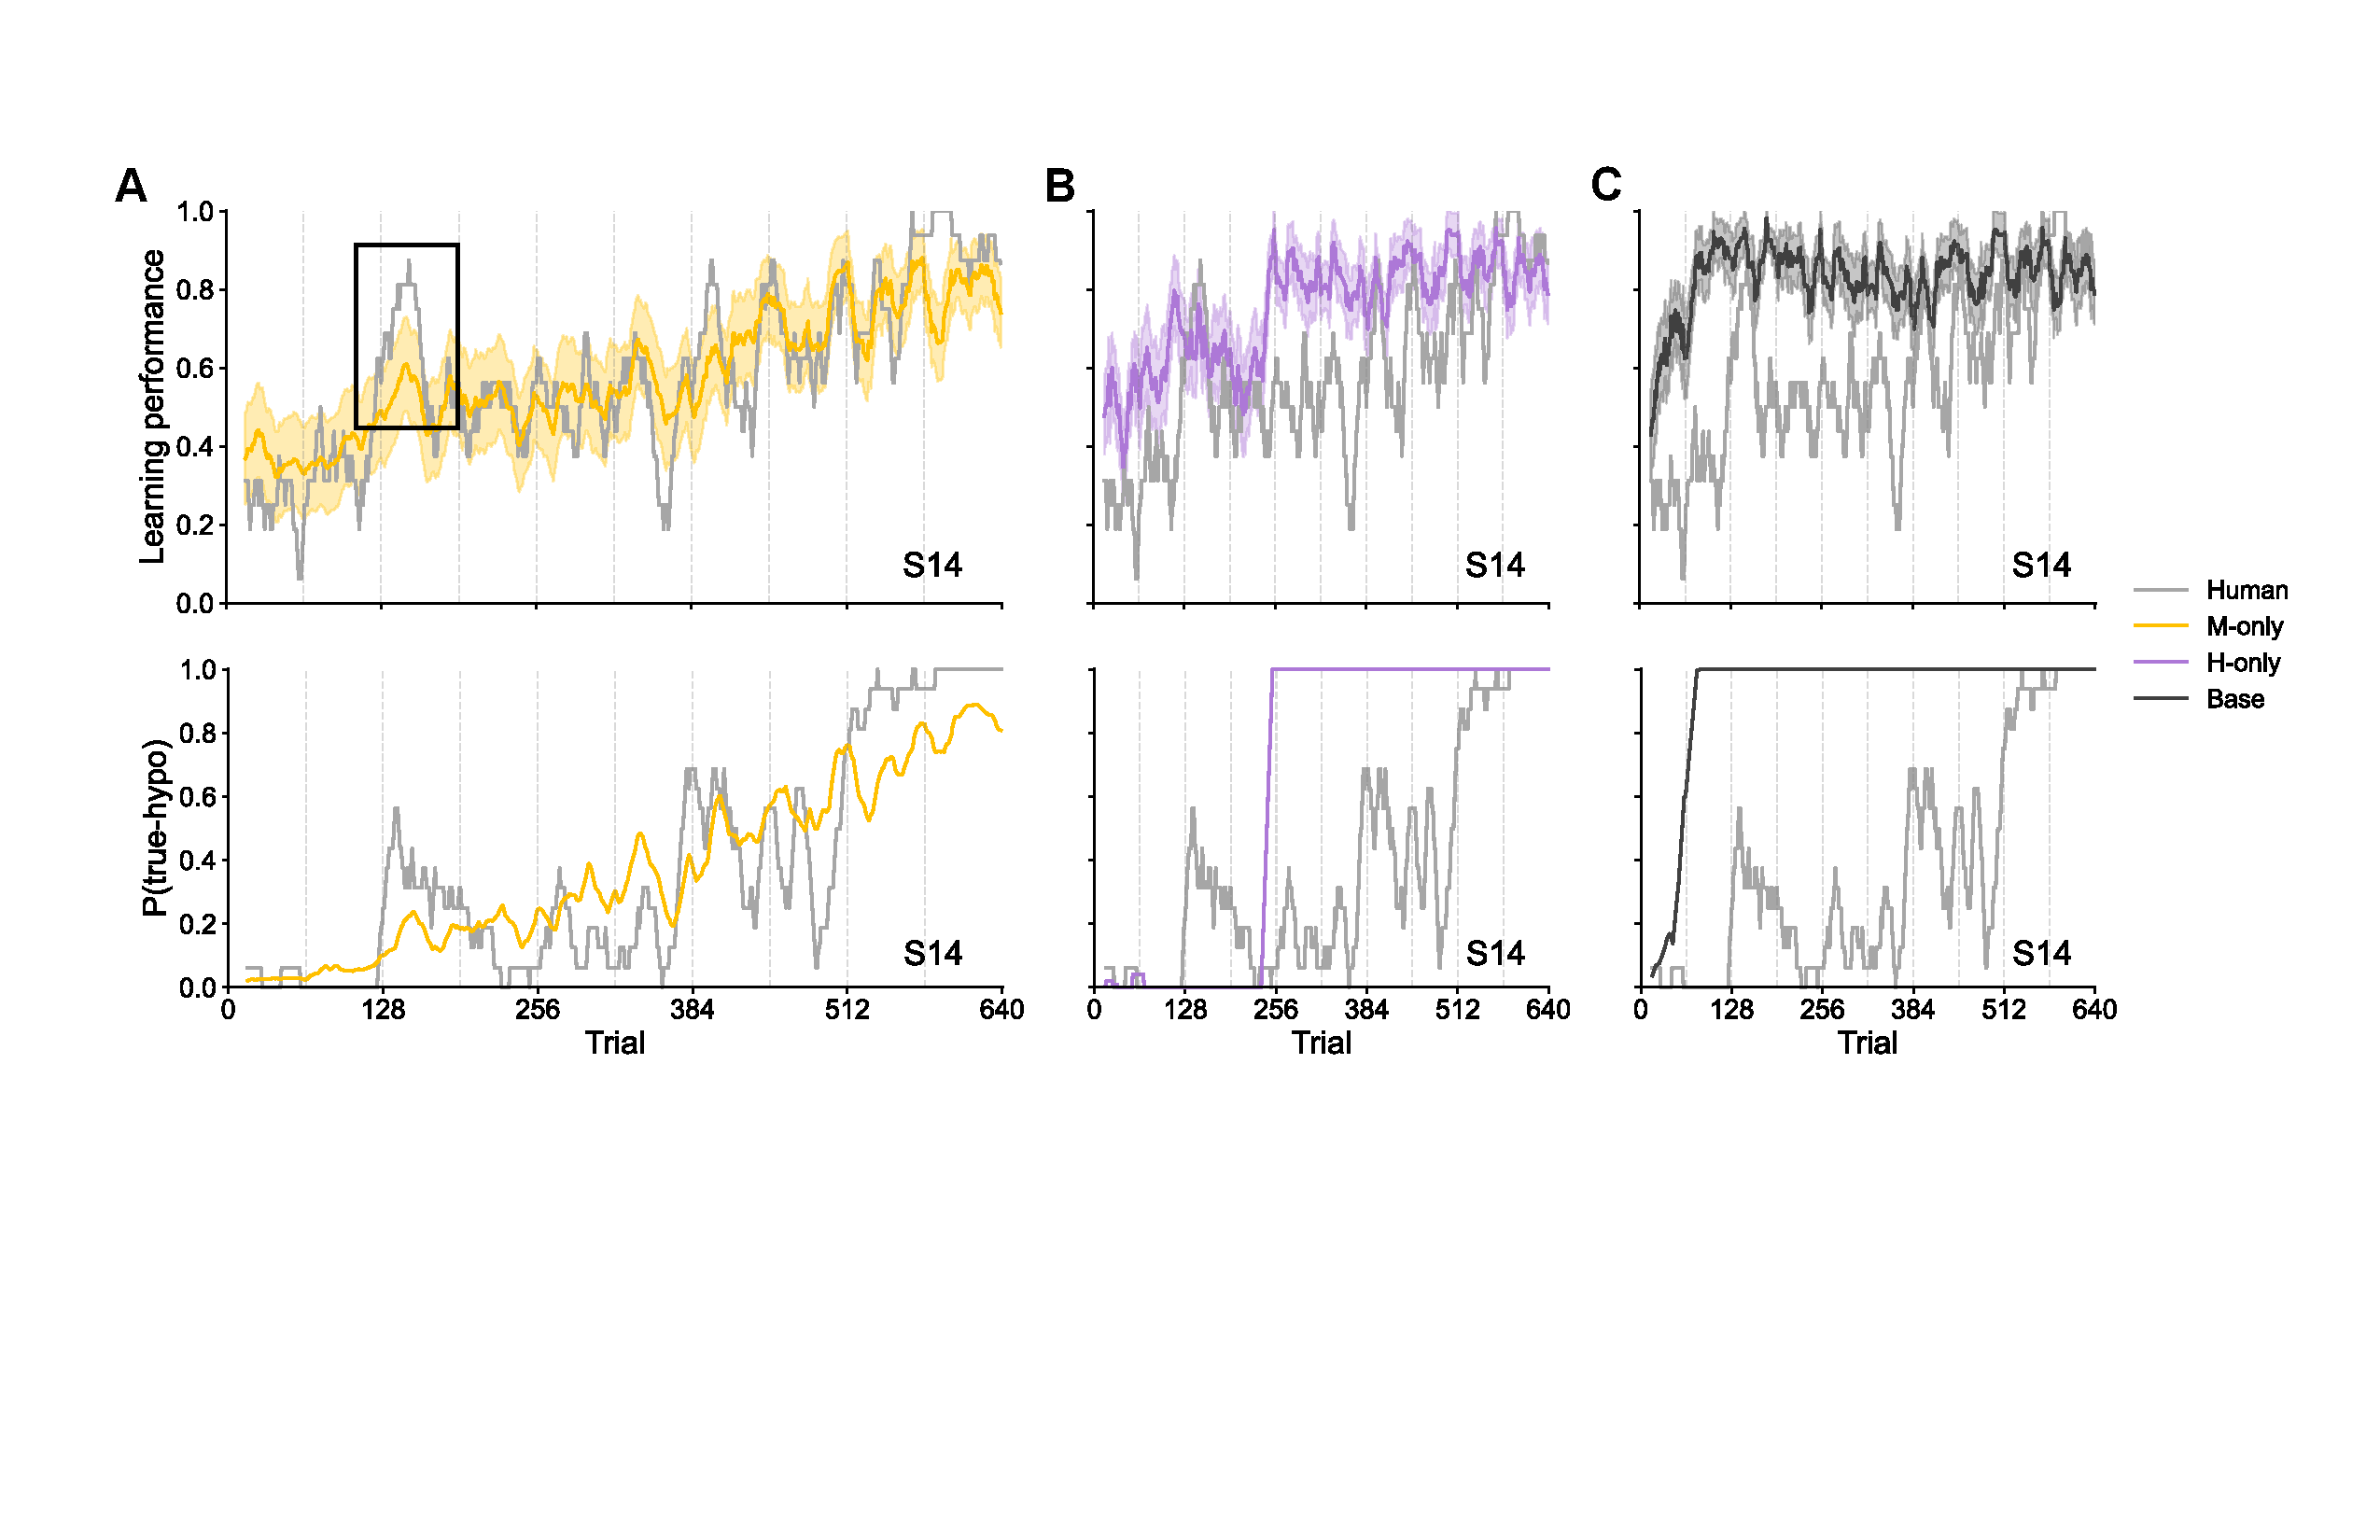
\includegraphics[width=1\textwidth, trim=2cm 8.5cm 1cm 3cm, clip]{figs/Figure4.pdf}  
  \caption{Behavioral and representational fits for two reduced model variants. \textbf{(A)} M-only model generally captures human-level behavioral accuracy but fails to align with participants’ internal hypothesis trajectories. \textbf{(B)} H-only model fails to reproduce both behavioral performance and internal dynamics, resembling the overly rapid convergence of the base model. \textbf{(C)} Base model’s trajectory illustrates near-optimal rule acquisition without bounded constraints.}
  \label{fig:4}
\end{figure}
% \vspace{1em}

Fig.~\ref{fig:4}A-B presents critical comparisons using two representative models from our ensemble: the M-model, which implements only the memory decay mechanisms, and the H-model, which includes only the hypothesis generator. These reduced variants were chosen to highlight two interesting cases. For the M-model, it predicts the overall trend of human overt behavior (see yellow vs. gray line) at a similar level to the HPM-model (Fig.~\ref{fig:3}C). However, its prediction on the internal hypothesis trajectory diverges significantly from participants’ verbal reports (see small panel in Fig.~\ref {fig:3}D). This dissociation highlights a critical point: modeling overt behavior alone proves insufficient – even good-level performance predictions may fundamentally misrepresent the internal processing. 
In contrast, the H-model (Fig.~\ref{fig:4}B) fails to reproduce both behavioral performance and internal hypothesis dynamics of the human learner. Its learning trajectory resembles that of the base model (Fig.~\ref{fig:4}C), which rapidly converges to the categorization rule. These results suggest that the local hypothesis sampling and rapid switching-and-testing are unnecessary for an agent with perfect memory and sensory fidelity. However, for humans, frequently switching among feature hypotheses in high-dimensional spaces may serve as a compensatory strategy to mitigate information loss (due to perceptual noise and memory decay), thereby increasing the chance of hitting the correct hypothesis. We explore this hypothesized compensatory mechanism in Section \ref{sec:4.2}. 



\subsection{Mechanistic explanations via modular analysis} \label{sec:4.2}
We analyze the hypothesis generator of HPM-model to understand how individuals develop their feature strategies during learning. Fig. ~\ref{fig:5}A shows that the amount of two strategies, stochastic exploration (in dark purple) and posterior-based exploitation (in light purple), generated as learning progresses (x-axis). Results of all participants are in Appendix B. This visualization reveals three distinct phases: Early phase, dominated by exploratory hypotheses, captures the initial random search in the feature space; Middle phase, exhibiting fluctuations between explorative vs. exploitative dominance, suggesting an adaptive arbitration between sampling novel vs. validating evidence-driven candidates; Late phase is increasingly governed by the posterior-based exploitation, indicating a convergence toward the correct rule via gradient-like refinement. 
Interestingly, we found a significant negative correlation between the length of the middle phase and participants’ memory capacity, as indexed by the fitted memory maintenance ($w_0$ parameter in memory module, see Section \ref{sec: model}.2) of HPM-model (Fig.~\ref {fig:5}B). As shown, participants with lower memory capacity tend to sustain the exploration-exploitation alternation for longer periods. This finding demonstrates a rational-bonded hypothesis selection: individuals with more limited memory engage in prolonged cycles of exploration and exploitation to compensate for information loss and ultimately converge on the correct feature hypothesis.


% \vspace{1em}
\begin{figure}[htp!]
  \centering
  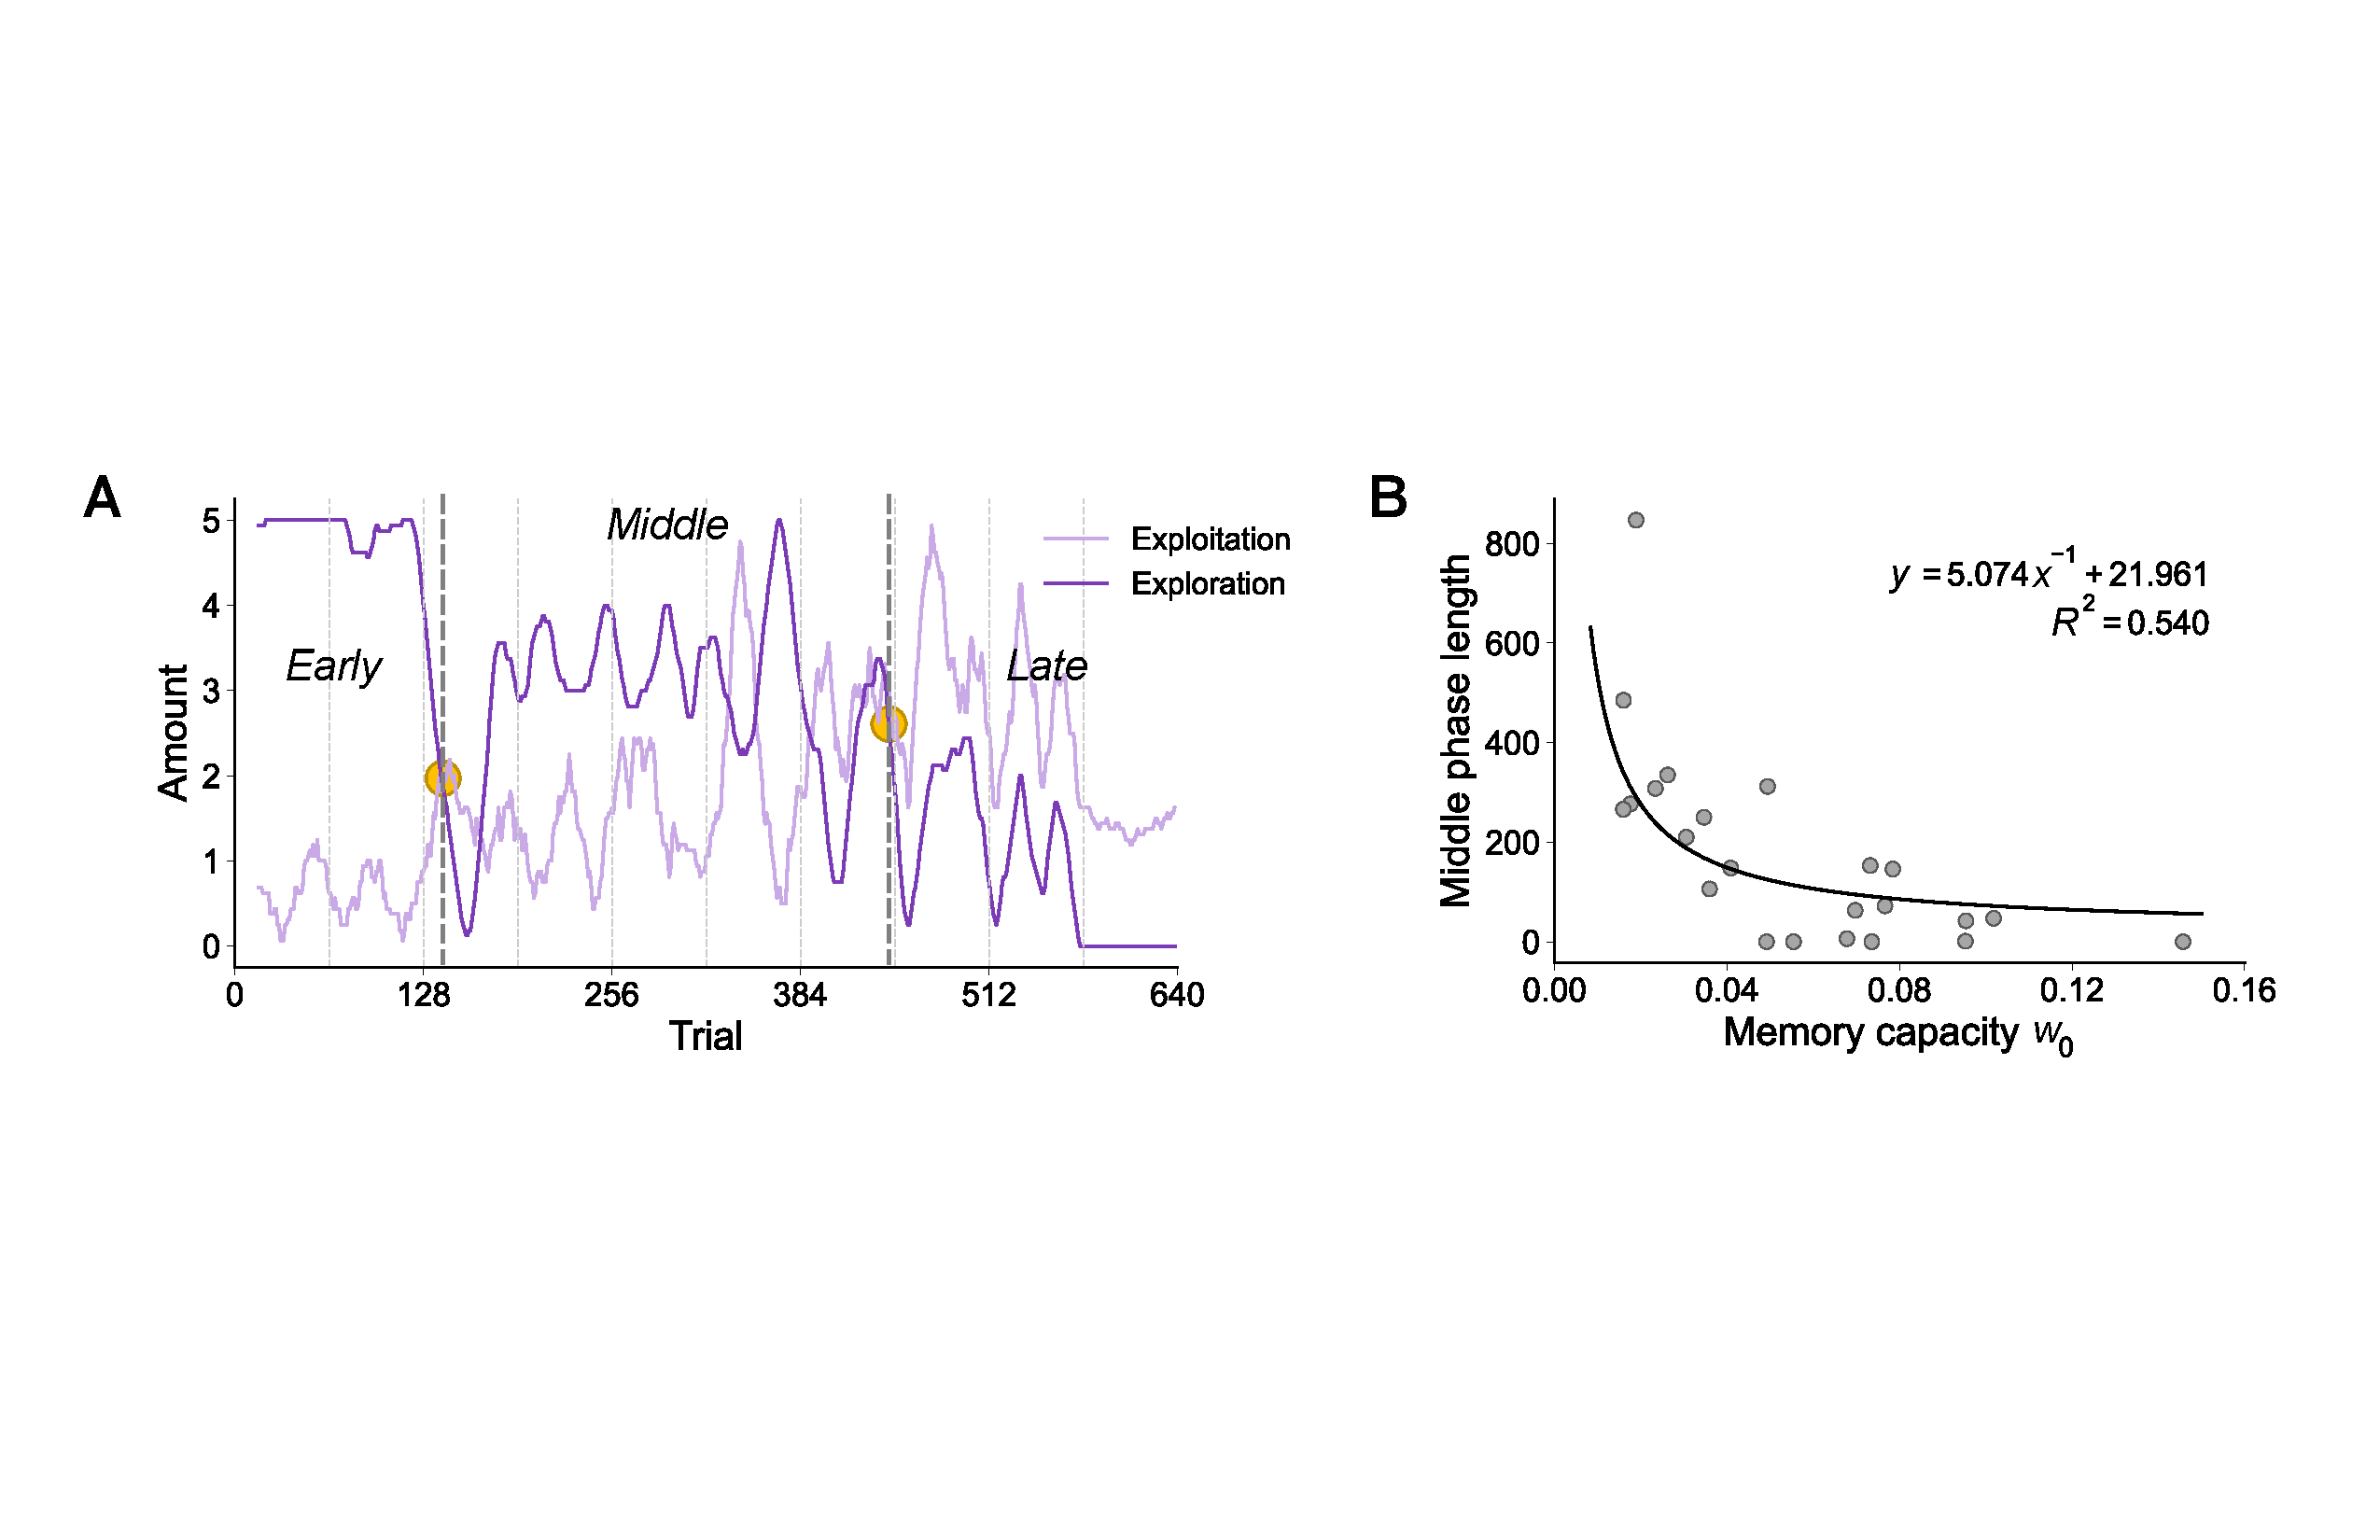
\includegraphics[width=1\textwidth, trim=0cm 8.5cm 0cm 8.5cm, clip]{figs/Figure5.pdf}  
  \caption{Dynamics of hypothesis selection strategies and their relation to memory capacity. \textbf{(A)} Temporal profiles of two strategies—stochastic exploration (dark purple) and posterior-based exploitation (light purple)—used by the HPM model across learning trials. \textbf{(B)} A significant negative correlation between the duration of the arbitration phase and individual memory capacity ($w_0$ from the memory module).}
  \label{fig:5}
\end{figure}
% \vspace{1em}